\subsection{Организация программного комплекса системы}
\label{sub:system-implementation:backend-architecture}

Основной целью в реализации программной части системы является чёткое разделение задач, что достигается следованием принципам чистой архитектуры. Это достигается путем разделения программного обеспечения на слои, где существует как минимум один слой для бизнес-правил, а другой~-- для интерфейсов. На сегодняшний это одно из самых популярных решений для разработки, так как обеспечивает читаемость, расширяемость, устойчивость и гибкость. Чистая архитектура помогает избежать проблем с зависимостями и разделить структуру программного комплекса на логические блоки. Ниже приведены основные преимущества системы, использующей такой подход.

\begin{itemize}
    \item независимость от фреймворков. Архитектура не зависит от существования некоторой библиотеки программного обеспечения с множеством функций. Это позволяет использовать такие фреймворки как инструменты, а не встраивать свою систему в их ограниченные рамки;
    \item тестируемость. Бизнес-правила можно тестировать без пользовательского интерфейса, базы данных, веб-сервера или любого другого внешнего элемента;
    \item независимость от пользовательского интерфейса. Пользовательский интерфейс можно легко изменить, не меняя остальную часть системы. Например, веб-интерфейс может быть заменен на консольный, без изменения бизнес-правил;
    \item независимость от базы данных, что позволяет заменить \textit{Oracle} или \textit{SQL Server} на \textit{MongoDB}, \textit{PostgreSQL}, \textit{MySQL} или что-то еще. Бизнес-правила не привязаны к базе данных.
\end{itemize}

Главный принцип чистой архитектуры~-- разделение приложения на уровни, каждый из которых выполняет свои задачи и является независимым от других слоев. Для реализации такого поведения необходимо придерживаться правила зависимостей. Диаграмма на рис.~\ref{fig:clean-architecture-diagram} наглядно отображает взаимосвязь слоёв приложения. Каждый из них представляет различные области программного обеспечения. По мере продвижения вглубь программное обеспечение становится все более абстрактным и включает в себя политики более высокого уровня. Самый внутренний круг~-- самый общий. Внешние круги~-- это механизмы и конкретные реализации. Внутренние круги~-- это правила, ограничения и политики~\cite{web_clean_architecture}.

\begin{figure}[h]
\centering
    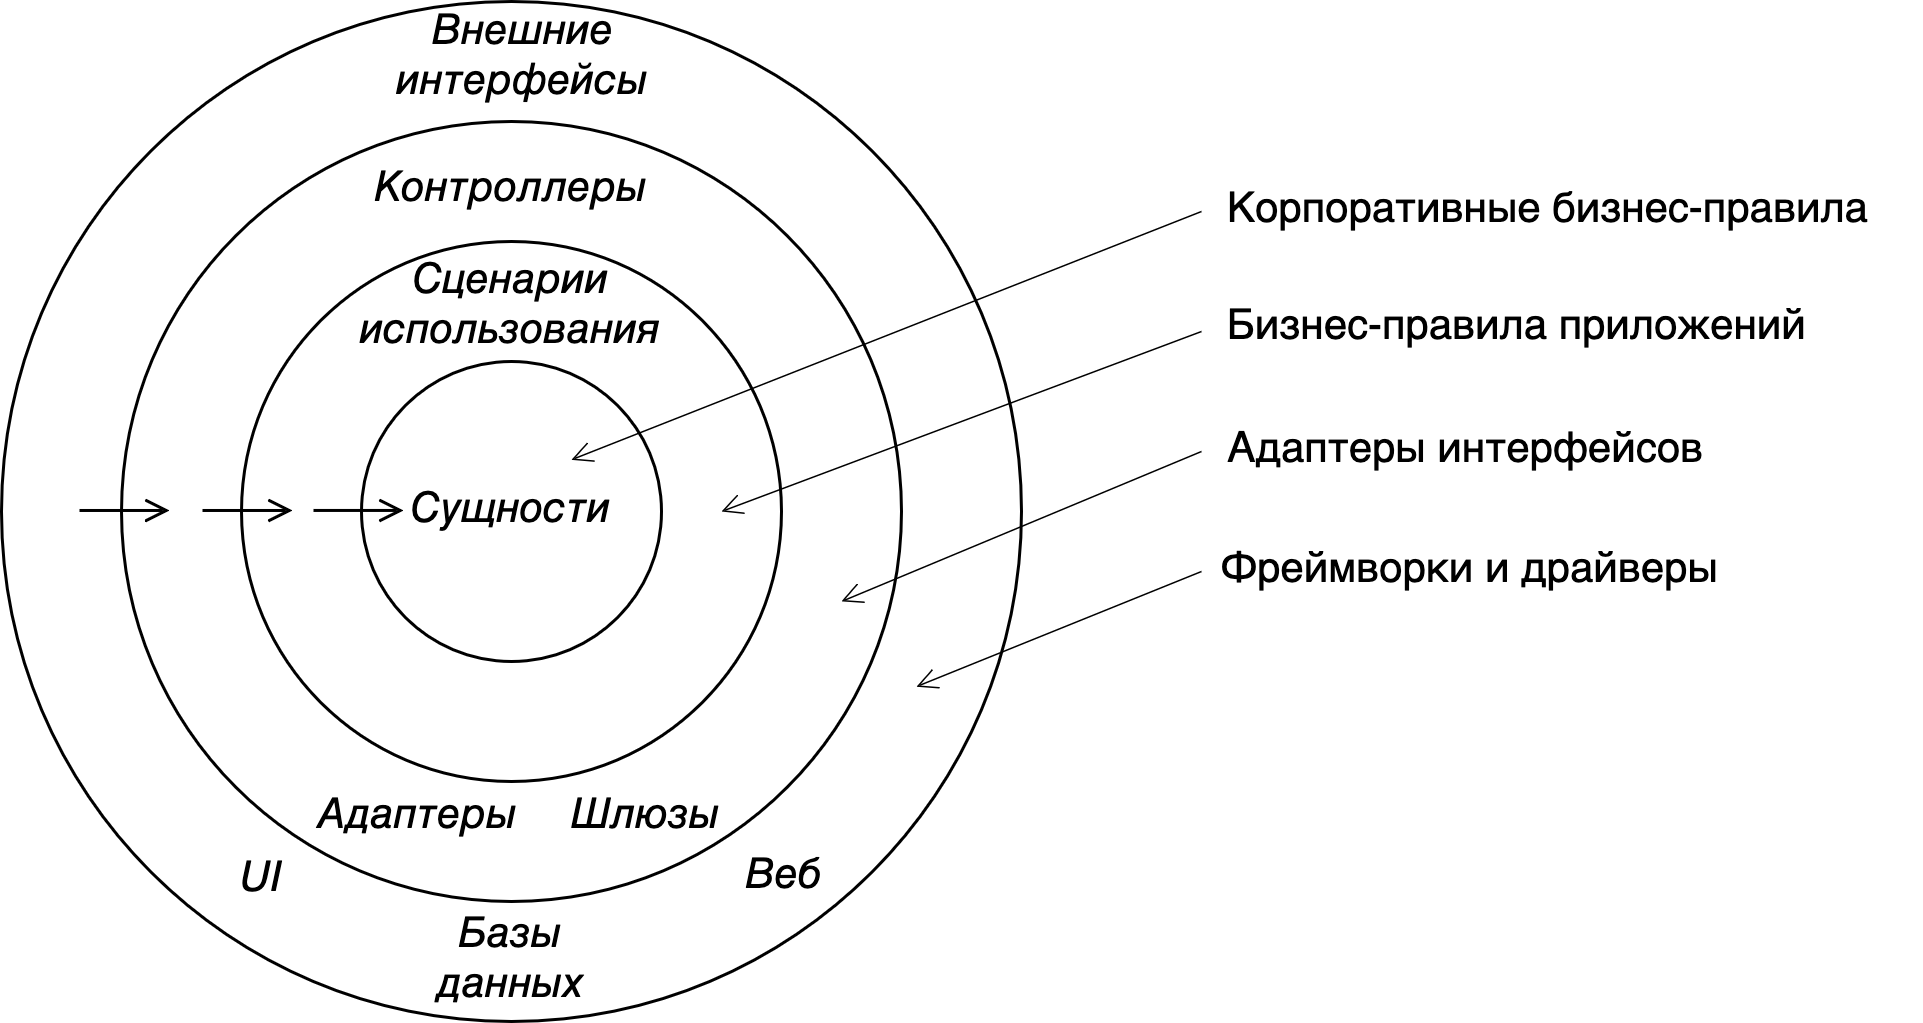
\includegraphics[width=0.9\linewidth]{assets/clean-architecture-diagram.png}
    \caption{Диаграмма взаимосвязи слоёв приложения}
    \label{fig:clean-architecture-diagram}
\end{figure}

\subsubsection{Правило зависимостей. }

Главным правилом, благодаря которому эта архитектура работает, является правило зависимостей (\textit{The Dependency Rule}). Это правило гласит, что зависимости исходного кода могут быть направлены только внутрь. Ничто во внутреннем круге не может знать что-либо о чем-то во внешнем круге. В частности, имя чего-то, объявленного во внешнем круге, не должно упоминаться в коде внутреннего круга. Это относится к функциям, классам, переменным и любым другим именованным программным объектам.

Таким же образом форматы данных, используемые во внешнем круге, не должны использоваться во внутреннем круге, особенно если эти форматы генерируются фреймворком во внешнем круге.

\subsubsection{Сущности. }

Сущности инкапсулируют бизнес-правила для всего предприятия. Сущность может быть объектом с методами, а может быть набором структур данных и функций. Это не имеет значения, если сущности могут использоваться различными приложениями на предприятии. Они с наименьшей вероятностью будут меняться при изменении чего-то внешнего. Никакие операционные изменения в конкретном приложении не должны влиять на слой сущностей. В листинге ниже представлена модель сущности сотрудника предприятия, реализованная с помощью класса данных (\textit{Dataclass}), предоставляемого встроенным в \textit{Python} модулем \textit{dataclasses}:

\begin{lstlisting}[style=pythonstyle]
class EmployeeRoleOption(StrEnum):
    employee = "EMPLOYEE"
    office_manager = "OFFICE_MANAGER"
    facility_manager = "FACILITY_MANAGER"
    it_support = "IT_SUPPORT"
    receptionist = "RECEPTIONIST"
    safety_officer = "SAFETY_OFFICER"
    hr = "HR"
    resource_manager = "RESOURCE_MANAGER"
    admin = "ADMIN"

@dataclass
class Employee:
    first_name: str
    last_name: str
    email: str
    department_id: UUID
    position_id: UUID
    professional_level_id: UUID
    phone_number: Optional[str] = None
    role: EmployeeRoleOption = EmployeeRoleOption.employee
    middle_name: Optional[str] = None
    picture: Optional[str] = None
    is_blocked: bool = False
    is_archived: bool = False
    created_at: datetime = field(default_factory=datetime.now)
    modified_at: datetime = field(default_factory=datetime.now)
    id: UUID = field(default_factory=uuid4)
\end{lstlisting}

Атрибут \textit{role} для модели сотрудника является объектом класса \textit{Employee\-Role\-Option}, наследованным от \textit{StrEnum}. Стоит отметить, что \textit{Dataclass} в \textit{Python} не предоставляет возможностей для проверки правильности с точки зрения бизнес-логики атрибутов класса, без явного переопределения метода \textit{\lstinline!__post_init__!}. Как упоминалось ранее, операции по проверке осуществляются во внешних слоях (интерфейсами и контроллерами).

\subsubsection{Сценарии использования. }

Программное обеспечение на этом уровне содержит бизнес-правила, специфичные для конкретного приложения. Оно инкапсулирует и реализует все сценарии использования системы, организуя поток данных к сущностям и от них, а также направляют эти сущности на использование бизнес-правил в масштабах предприятия для достижения целей сценария использования.

При этом не ожидается, что изменения в этом слое повлияют на сущности или что на этот слой повлияют изменения внешних факторов, таких как база данных, пользовательский интерфейс или любой из общих фреймворков. Этот слой изолирован от подобных проблем.

Тем не менее, ожидается, что изменения в работе приложения повлияют на сценарии использования и, следовательно, на программное обеспечение в этом слое. Если детали сценария использования изменятся, то код в этом слое обязательно будет затронут. Пример реализованного для рассматриваемой системы сценария использования приведен в следующем листинге:

\begin{lstlisting}[style=pythonstyle]
class ApproveWorkspaceOccupationRequestUseCase:
    def __init__(
        self,
        employee_repository: EmployeeRepository,
        workspace_repository: WorkspaceRepository,
        workspace_occupation_repository: WorkspaceOccupationRepository,
        occupation_request_repository: OccupationRequestRepository,
    ):
        self._employee_repository = employee_repository
        self._workspace_repository = workspace_repository
        self._workspace_occupation_repository = workspace_occupation_repository
        self._occupation_request_repository = occupation_request_repository

    async def __call__(
        self, request_id: UUID, approver_employee: Employee, approver_comment: str
    ) -> None:
        occupation_request = await self._occupation_request_repository.get(
            id=request_id
        )
        await self._validate_occupation_request(occupation_request)

        requested_workspace = await self._workspace_repository.get(
            id=occupation_request.object_id
        )
        self._validate_workspace(requested_workspace)

        occupation = WorkspaceOccupation(
            type=occupation_request.occupation_type,
            workspace_id=occupation_request.object_id,
            employee_id=occupation_request.requester_employee_id,
            start_date=occupation_request.start_date,
            end_date=occupation_request.end_date,
        )
        occupation = await self._workspace_occupation_repository.create(occupation)
        
        occupation_request.status = OccupationRequestStatusOption.approved
        occupation_request.approver_employee_id = approver_employee.id
        occupation_request.approver_comment = approver_comment
        occupation_request.modified_at = datetime.now()
        await self._occupation_request_repository.update(occupation_request)

        await self._workspace_repository.update(
            id=occupation_request.object_id,
            status=WorkspaceStatusOption.occupied,
            modified_at=datetime.now(),
        )

    async def _validate_occupation_request(
        self, occupation_request: OccupationRequest
    ) -> None:
        if occupation_request.is_archived:
            raise OccupationRequestArchivedError
        if occupation_request.status != OccupationRequestStatusOption.in_progress:
            raise OccupationRequestInvalidStatusError(
                f"Occupation request status is {occupation_request.status}, expected IN_PROGRESS"
            )
        if occupation_request.request_type != OccupationRequestTypeOption.workspace:
            raise OccupationRequestInvalidTypeError(
                f"Occupation request type is {occupation_request.request_type}, expected WORKSPACE"
            )
        if occupation_request.start_date > occupation_request.end_date:
            raise OccupationRequestInvalidDateError(
                f"Occupation request start date {occupation_request.start_date} is after end date {occupation_request.end_date}"
            )

        existing_occupation = await self._workspace_occupation_repository.get_current()
        if existing_occupation:
            raise OccupationRequestAlreadyOccupiedError(
                "There is already an existing occupation for this workspace"
            )

        requester_employee = await self._employee_repository.get(
            id=occupation_request.requester_employee_id
        )
        if requester_employee.is_archived:
            raise EmployeeArchivedError(f"Requested employee is archived")
        if requester_employee.is_blocked:
            raise EmployeeBlockedError(f"Requested employee is blocked")

    def _validate_workspace(self, workspace: Workspace) -> None:
        if not workspace:
            raise WorkspaceDoesNotExistError(
                f"Requested workspace with ID {occupation_request.object_id} does not exist"
            )
        if workspace.is_archived:
            raise WorkspaceArchivedError
        if workspace.status != WorkspaceStatusOption.free:
            raise WorkspaceInvalidStatusError(f"Requested workspace is not free")
\end{lstlisting}

Класс \textit{ApproveWorkspaceOccupationRequestUseCase}, содержащий реализацию конкретной части бизнес-логики, содержит атрибуты, являющиеся объектами конкретных реализаций контроллеров, в данном случае~-- репозитории сущностей. Для аннотации типов используются абстрактные классы соответствующих адаптеров. В качестве примера рассмотрим репозиторий сотрудников, где \textit{EmployeeRepository}~-- абстрактный класс, содержащий определения основных методов для работы с объектами типа \textit{Employee}, а класс \textit{PostgresEmployeeRepository} является конкретной его реализацией для базы данных \textit{PostgreSQL}. Для юнит-тестирования принято также иметь классы для хранения объектов в памяти, например, для рассмотренного случая класс \textit{InMemoryEmployeeRepository} реализует эту возможность.

Таким образом, принципы объектно-ориентированного программирования (ООП) обеспечивают гибкость, модульность и тестируемость системы. Бизнес-логика сценария использования инкапсулирована внутри класса. Внешние зависимости передаются через конструктор, что скрывает детали их реализации от основного кода.

Использование абстрактных классов позволяет отделить определение от конкретной реализации, что соответствует принципу зависимости от абстракций (\textit{DIP}). Класс \textit{ApproveWorkspaceOccupationRequestUseCase} отвечает только за утверждение запросов, а репозитории — за работу с даннымы, что соответствует принципу единственной ответственности (\textit{SRP}). Система открыта для расширения (можно добавить новые репозитории для других СУБД), но закрыта для модификации, что соответствует принципу открытости/закрытости (\textit{OCP}).

Пример с репозиториями иллюстрирует, как абстракции и инъекция зависимостей делают систему адаптируемой к изменениям инфраструктуры (аппаратной или программной).

\subsubsection{Адаптеры интерфейсов. }

Программное обеспечение этого слоя представляет собой набор адаптеров, которые преобразуют данные из формата, наиболее удобного для сценариев использования и сущностей, в формат, наиболее удобный для какого-либо внешнего слоя, например базы данных или \textit{Web}. Представления и контроллеры~-- все они находятся здесь. Модели~-- это просто структуры данных, которые передаются от контроллеров к сценариям использования, а затем обратно от сценариев использования к представлениям~\cite{book_clean_architecture}. Этот слой реализует паттерн проектирования \textit{Adapter}, обеспечивая взаимодействие между абстрактной бизнес-логикой и конкретными технологическими решениями.

Аналогично, в этом слое данные преобразуются из формы, наиболее удобной для сущностей и сценариев использования, в форму, наиболее удобную для любого используемого фреймворка или базы данных. Кроме того, данный слой обычно отвечает за проверку и сериализацию входящих и исходящих данных. В нашем случае эта функциональность делегирована \textit{FastAPI} (в частности, \textit{Pydantic}). Для разрешения зависимостей используется встроенный в \textit{FastAPI} механизм инъекции зависимостей~\cite{book_lubanovich_fastapi} (\textit{Dependency injection}).

Для рассмотренного ранее примера, различные репозитории для управления данными являются адаптерами в контексте архитектуры. Кроме того, адаптерами также могут выступать различные инструменты для интеграции сторонних систем, например для контроля посещаемости, или инструменты аутентификации. Схема взаимосвязи компонентов для рассмотренного примера утверждения запроса на бронирование представлена на рис.~\ref{fig:system-implementation:software:clean-architecture-adapter-components}.

\begin{figure}[h]
\centering
    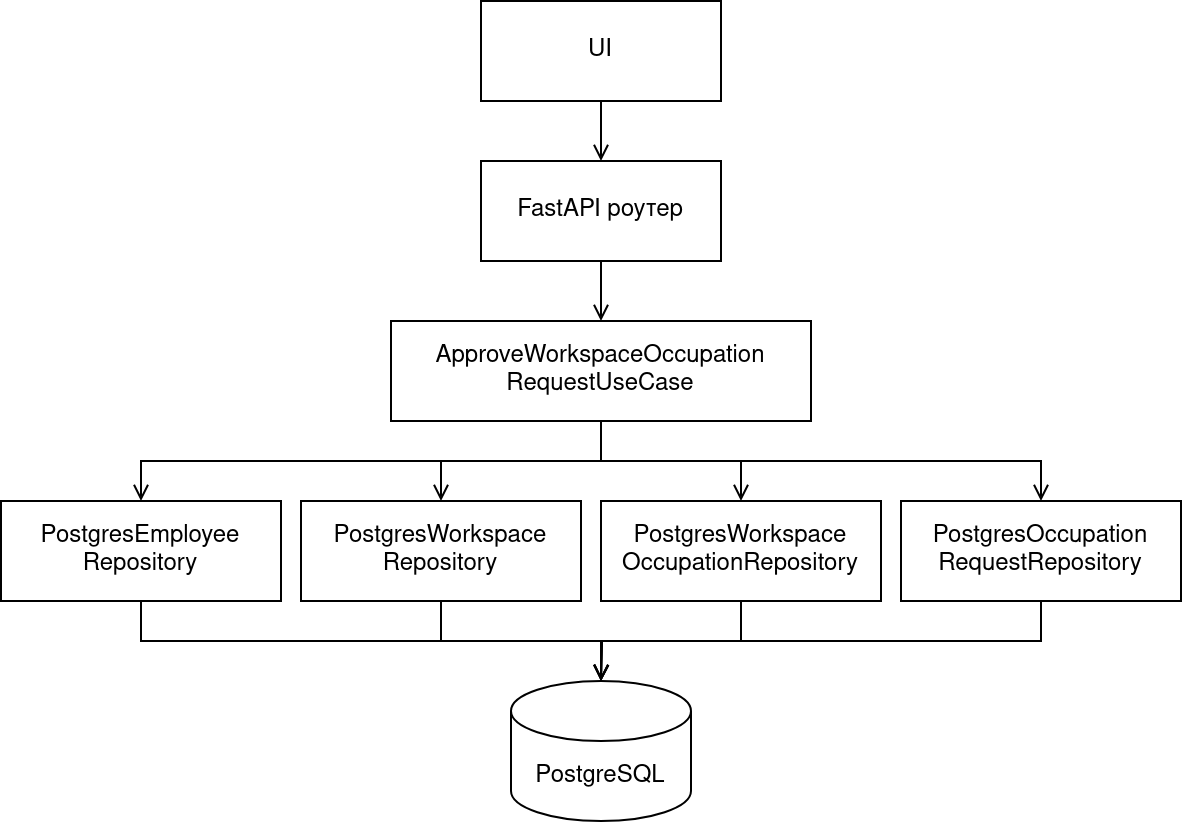
\includegraphics[width=0.9\linewidth]{assets/clean-architecture-adapter-components.png}
    \caption{Схема взаимосвязи компонентов для процесса утверждения запроса на бронирование}
    \label{fig:system-implementation:software:clean-architecture-adapter-components}
\end{figure}

Адаптеры выполняют три ключевые функции:

\begin{enumerate}
    \item Трансляция данных: преобразование структур данных между внутренним (доменным) и внешним (техническим) представлением. Например, объект сущности \textit{Employee} сериализуется в \textit{JSON} для \textit{REST API} или в строку \textit{SQL} для \textit{PostgreSQL}.
    \item Интеграция с внешними системами: реализация протоколов взаимодействия с базами данных, сторонними \textit{API}, инструментами аутентификации (\textit{OAuth2}, \textit{JWT}) или механизмами кэширования (\textit{Redis}).
    \item Изоляция изменений: сокрытие деталей работы внешних компонентов от бизнес-логики. Замена базы данных, к примеру, потребует лишь создания нового адаптера без модификации кода сценария использования.
\end{enumerate}

В системе можно выделить несколько категорий адаптеров:

\begin{itemize}
    \item контроллеры \textit{API}, например, \textit{FastAPI}-роутеры выступают адаптерами для \textit{HTTP}. Они принимают запросы и преобразуют их в \textit{DTO} (\textit{Data Transfer Objects}) с помощью \textit{Pydantic}, вызывают сценарии использования, передавая параметры в доменном формате и сериализуют результаты в ответы \textit{API};
    \item интеграционные адаптеры, которые являются классами для работы с внешними сервисами, например адаптер для отправки уведомлений может поддерживать как \textit{SMTP}, так и \textit{Slack}-каналы;
    \item репозитории, являющиеся классами вроде \textit{Postgres\-Employee\-Re\-po\-si\-to\-ry}, как показано в листинге ниже, которые реализуют интерфейс \textit{Employee\-Re\-po\-si\-to\-ry}, абстрагируя доступ к данным. Они инкапсулируют \textit{SQL}-запросы, \textit{ORM}-модели и транзакции.
\end{itemize}

\begin{lstlisting}[style=pythonstyle]
class EmployeeRepository(ABC):
    @abstractmethod
    async def get(self, **filters: Any) -> Employee | None:
        pass

    @abstractmethod
    async def get_many(
        self,
        filters: dict | None = None,
        or_filters: dict | None = None,
        or_ilike_filters: dict | None = None,
        sort_by: (Literal["id", "first_name", "last_name", "email", "phone_number", "created_at", "modified_at"] | None) = "id",
        order_by: Literal["asc", "desc"] | None = "asc",
        page: int = 1,
        limit: int = 100,
    ) -> tuple[int, list[Employee]]:
        pass

    @abstractmethod
    async def create(self, employee: Employee) -> Employee:
        pass

    @abstractmethod
    async def update(self, updated_user: Employee, **filters: Any) -> Employee | None:
        pass

    @abstractmethod
    async def delete(self, **filters) -> None:
        pass
\end{lstlisting}

Для оптимизации работы с СУБД \textit{PostgreSQL} используются такие подходы как: пулы соединений (\textit{asyncpg.Pool}) для снижения накладных расходов, выполнение асинхронных запросов через \textit{SQLAlchemy Core}, избегая блокировки \textit{event loop} и индексирование таблиц по часто используемым в выборках полям. Пример запроса получения данных сотрудника из базы данных \textit{PostgreSQL}, используя \textit{SQLAlchemy}, представлен в листинге ниже:

\begin{lstlisting}[style=pythonstyle]
async def get(self, _or: bool = False, **filters: Any) -> User | None:
    try:
        query = select(UserModel)
        if _or:
            query = query.filter(or_(*[getattr(UserModel, key) == value for key, value in filters.items()]))
        else:
            query = query.filter_by(**filters)
        user = await self.session.execute(query)
        user = user.scalars().first()
        return self.__to_user_entity(user) if user else None
    except Exception as e:
        raise DatabaseError(e)
\end{lstlisting}

Интеграция с \textit{RabbitMQ} выполнена с использованием адаптера для брокера сообщений. Его задачами являются: сериализация доменных события (например, \textit{WorkspaceOccupiedEvent}) в \textit{JSON}, отправка сообщений в очередь \textit{\lstinline!workspace_events!}, обработка подтверждения доставки и повторные попытки. В листинге ниже представлен класс \textit{RabbitMQEventPublisher} для публикации событий в очередь \textit{RabbitMQ}:

\begin{lstlisting}[style=pythonstyle]
class RabbitMQEventPublisher:
    def __init__(self, channel: aio_pika.Channel):
        self._channel = channel

    async def publish(self, event: DomainEvent) -> None:
        message = aio_pika.Message(
            body=event.json().encode(),
            headers={"event_type": event.__class__.__name__}
        )
        await self._channel.default_exchange.publish(
            message, routing_key="workspace_events"
        )
\end{lstlisting}

Таким образом, адаптеры интерфейсов служат «мостом» между стабильным ядром системы и изменчивым внешним окружением.

\subsubsection{Фреймворки и драйверы. }

Внешний слой системы представляет собой инфраструктурные компоненты, которые обеспечивают взаимодействие приложения с внешним миром. Этот слой включает:

\begin{itemize}
    \item веб-фреймворки (для рассматриваемой системы~-- \textit{FastAPI}), обрабатывающие \textit{HTTP}-запросы и формирующие ответы;
    \item СУБД и драйверы (\textit{PostgreSQL} через \textit{asyncpg}, \textit{SQLAlchemy Core}), управляющие хранением данных;
    \item брокеры сообщений (для рассматриваемой системы~-- \textit{RabbitMQ}), обеспечивающие асинхронную коммуникацию между сервисами;
    \item сторонние \textit{API} (платежные шлюзы, сервисы аутентификации), интегрируемые через \textit{REST} или \textit{gRPC};
\end{itemize}

Операции пути (роутеры) \textit{FastAPI} выступают точкой входа для внешних запросов. Они выполняют проверку входных данных через \textit{Pydantic}, внедряют зависимости (\textit{Use Cases}, репозитории) через механизм \textit{DI}, преобразуют исключения доменного слоя в \textit{HTTP}-статусы (например, \textit{EmployeeNotFoundError} в \textit{HTTP}-статус 404 с соответствующим сообщением). В листинге ниже представлена операция пути \textit{FastAPI} для обновления данных сотрудника:

\begin{lstlisting}[style=pythonstyle]
@router.patch("/employee/{employee_id}", status_code=status.HTTP_200_OK, response_model=EmployeeOut)
@role_required([EmployeeRoleOption.hr])
async def update_employee(
    employee_id: UUID,
    data: EmployeeUpdate,
    use_case: Annotated[UpdateEmployeeUseCase, Depends(get_update_employee_use_case)],
    employee: Employee = Depends(get_logged_employee),
) -> Employee:
    return await use_case(employee_id, data.model_dump(exclude_unset=True))
\end{lstlisting}

Критерии выбора инструментов включают в себя несколько важных условий, главным из которых является совместимость с асинхронной моделью, а именно поддержка \textit{async/await} (например, использование \textit{asyncpg} вместо \textit{psycopg2} для взаимодействия с базой данных \textit{PostgreSQL}), производительность, безопасность (например, встроенная защита от \textit{SQL}-инъекций в \textit{SQLAlchemy}, \textit{OAuth2} в \textit{FastAPI}~\cite{book_lubanovich_fastapi}).

Таким образом, фреймворки и драйверы, будучи технической реализацией внешнего слоя, обеспечивают эффективное взаимодействие с внешними системами без нарушения границ домена, масштабируемость за счет асинхронности и выделения ресурсов, надёжность через обработку ошибок и транзакции.

Пример потока данных по всем архитектурным слоям логики системы показан на рис.~\ref{fig:system-implementation:software:clean-architecture-data-flow}.

\begin{figure}[h]
\centering
    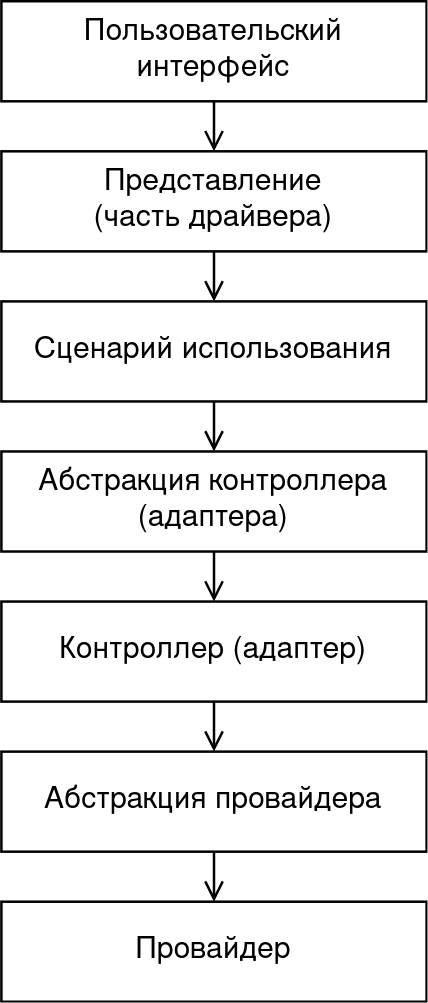
\includegraphics[width=0.33\linewidth]{assets/clean-architecture-data-flow.png}
    \caption{Схема потоков данных в системе}
    \label{fig:system-implementation:software:clean-architecture-data-flow}
\end{figure}

Подводя итоги, можно отметить, что применение принципов чистой архитектуры в \textit{Python}-проектах обладает рядом значимых преимуществ, хотя и не лишено определённых сложностей. Главным достоинством такого подхода является независимость от сторонних библиотек и фреймворков, что позволяет избежать навязывания их структуры и сохранить гибкость разработки. Компоненты приложения становятся слабосвязанными, что упрощает их замену~-- например, переход на другую базу данных или инструмент требует минимальных изменений, не затрагивая ядро системы. Это также значительно повышает тестируемость: добавление новой функциональности и её проверка становятся проще благодаря чёткому разделению слоёв. Кроме того, проект приобретает прозрачную и масштабируемую структуру, где каждый элемент имеет строго определённую зону ответственности.

Достичь этих результатов помогает комбинация двух ключевых концепций: внедрения зависимостей и инверсии управления. Например, в рассмотренном проекте адаптеры, такие как \textit{EmployeeRepository}, внедряются в сценарии использования, что позволяет абстрагироваться от конкретной реализации. Вместо прямого использования репозитория в бизнес-логике применяются абстрактные классы, задающие интерфейсы для взаимодействия. Это обеспечивает соблюдение границ между слоями архитектуры.

Однако у подхода есть и недостатки. На первый взгляд принципы чистой архитектуры могут показаться сложными из-за необходимости глубокого понимания абстракций и инверсии зависимостей, а структура проекта~-- избыточно громоздкой на первых этапах. Кроме того, декомпозиция и соблюдение строгой изоляции компонентов неизбежно ведут к увеличению объёма кода, что требует дополнительных усилий при разработке. Тем не менее, долгосрочные преимущества в виде поддерживаемости, гибкости и устойчивости к изменениям часто перевешивают эти трудности, особенно в крупных и долгоживущих проектах.
